\section{Обоснование решения}
\subsection{Терминология}
Определим ряд терминов, которые будут использоваться в данной работе:
\begin{itemize}
    \item GoClown --- программный продукт, реализованный в рамках данной работы.  
    \item Приложение --- сервис, тестируемый с помощью GoClown.  
    \item Внешние сервисы --- сервисы, с которыми взаимодействует приложение,
        и чье поведение имитируется GoClown.  
    \item Файл захвата --- запись сетевого взаимодействия приложения с внешними
        сервисами.  
    \item Сессия --- одиночный перид сетевого взаимодействия между сервисами.  
    \item Детерминированность системы --- свойство, означающее, что при
        повторении сценария взаимодействия внешнее поведение приложения
        не изменится.  
\end{itemize}

\subsection{Постановка задачи}
В компании Acronis системы, связанные с обработкой пользовательских учетных
записей, покупок, и метаданных, ассоциированных с пользователем были разработаны
в первой половине 2000-х годов на языке Perl, и, в силу быстрого развития
компании, основным приоритетом являлось скорее быстрое добавление нового
функционала, нежели строгая гарантия работы существующего. По этой причине не
было уделено должного внимания тестированию кода. На данный момент системы
находятся в режиме поддержки, и ограниченное число разработчиков не позволяет
уделять заметное время тестированию существующего кода способами, отличными от
разовых ручных проверок. Проблема, вызываемая этим усиливается устаревшими
версиями операционных систем виртуальных машин, на которых развернуто это
программное обеспечение. Из соображений безопасности было принято решение
перенести все системы на новые версии ОС с использованием виртуализации на
уровне ядра Docker. Данный процесс плохо автоматизирован, и требует большого
количества ручных проверок на предмет корректности функционирования системы
в новом окружении. В связи с этим возникает вопрос автоматизации обнаружения
дефектов при переносе системы без модификации исходного кода программного
обеспечения.

\subsection{Современные подходы к автоматическому тестированию}
Наиболее распространенное и хорошо изученное решение для тестирования
программных комплексов и приложений, состоящих из множества взаимодействующих
сервисов --- обнаружение аномалий в сетевых взаимодействиях и в процессе
исполнения программ~\cite{bohmer}. Данный подход хорошо себя зарекомендовал, но
он опирается на то, что система хорошо разделена на компоненты, что является
достаточно сильным требованием к качеству разработки, и что может не выполняться
для старых систем, созданных до появления хорошо отлаженных принципов разработки.

Идея применения такого способа тестирования к монолитному приложению,
работающему в пределах одного сервера достаточно интересна, но на практике она
накладывает достаточно много ограничений на скорость в силе ухудшения или
полного отключения оптимизаций интерпретатора или компилятора языка.

Еще одним подходом к тестированию является так называемое тестирование ''черного
ящика''. В этой методологии компоненты тестируются без каких-либо предположений
об их внутреннем устройстве, рассматривая только внешнее их
поведение~\cite{ahmed}. Правда обычно подразумевается, что тесты составляются
вручную, но они рассматривают лишь результаты операций публичных интерфейсов
модулей. В рамках такого подхода реализована утилита GoReplay, способная
повторять произвольные входящие HTTP-запросы, проверяя ответы сервисов. Это
позволяет использовать входные данные, получаемые непосредственно в процессе
эксплуатации, что дает возможность гораздо более реалистичные тесты нежели
синтетические и умозрительные. Но у GoReplay обладает несколькими критичными
ограничениями, делающими его недостаточно гибким для использования в рамках
поставленной задачи:
\begin{itemize}
    \item Бесплатная версия GoReplay не поддерживает бинарные протоколы, что не
дает возможности проверять взаимодействие с базами данных и схожими сервисами.  
    \item GoReplay требует наличия запущенной копии рабочего предложения для
снятия трафика, что может быть затруднительно в случае устаревших версий ОС.  
    \item GoReplay тестирует соединения в режиме ''многие к одному'', позволяя
отправить множество запросов проверяемому сервису, но не позволяя тестировать
общения одного сервиса и многих, к кому он обращается.  
\end{itemize}

\subsection{Специфика языка программирования Perl}
Язык программирования Perl обаладает некоторыми уникальными свойствами, которые
очень затрудняют статический анализ и генерацию тестов на его основе. В
частности, статический анализ языка Perl --- задача невычислимая в общем виде, и
не представляется возможным понять, что делает произвольный код на языке
программирования Perl. В силу этого использование любого автоматического
тестирования, основанного на анализе исходного кода программы исключается.
По этой причине решение для тестирования, представленное в данной работе,
должно быть наиболее абстрагировано от конкретных деталей языка. Это позволит
избежать ложных предположений о структуре программ.

\subsection{Выбор подхода}
В силу наличия требования на максимальное отделение способа тестирования от
используемого языка программирования, используемых библиотек и дополнительного
программного обеспечения, данная работа посвящена изучению подхода тестирования
''черного ящика'', путем проверки взаимодействия приложения с внешними сервисами,
то есть сервисами, находящимися на других серверах, такие как базы данных и
сервисы для удаленного вызова функций (RPC). Тестироваться будет взаимодействие
по протоколу TCP по причине того, что его используют все рассматриваемые
системы.

\subsection{Взаимодействие по протоколу UDP}
Протокол UDP пересылает датаграммы --- пакеты данных определенной длины,
отправляемые и принимаемые без контроля приема и повторений.  UDP-датаграммы
могут приходить повторно, теряться, или приходить с запозданием. Подход к
протоколу взаимодействия приложения со внешними сервисами, как с черным ящиком,
не позволяет анализировать, является ли данное UDP-сообщением отправленным и
полученным в правильный момент времени, что в свою очередь затрудняет построение
такого же диалога, как с TCP. Также как и с TCP, сложные протоколы, построенные
поверх (например, QUIC~\cite{quic}) не могут быть повторены наивным методом.

\subsection{Требования к тестируемой системе}
Основной фокус работы, как упоминалось выше, --- доказательство корректности
системы при изменении способа разворачивания системы, но без изменений в
исходном коде, меняющих взаимодействие с внешним миром.
Так как приложение тестируется путем повторения TCP диалога, также
предполагается, что система обладает детерминированностью, то есть
одинаковая последовательность данных от инициатора запроса (тестируемого
приложения) порождает одинаковую последовательность данных от адресата. Это
исключает мультиплексирование в пределах сессии, что активно используется,
например, в HTTP/2, использование случайных чисел, что исключает, например,
криптографические приложения и приложения, использующие шифрованные каналы
связи.  Данное ограничение валидно для простых HTTP/1.1 REST сервисов, которые
открывают новые соединения к базе данных в процессе обработки одного запроса.
Еще одну проблему при повторении трафика создает работа тестируемого
приложения в несколько потоков. Это может приводить к состоянию гонки при
повторном тестировании и нарушать детерминированность всей системы.
Пример валидной системы представлен на \autoref{fig:service_diagram}.

\begin{figure}[H]
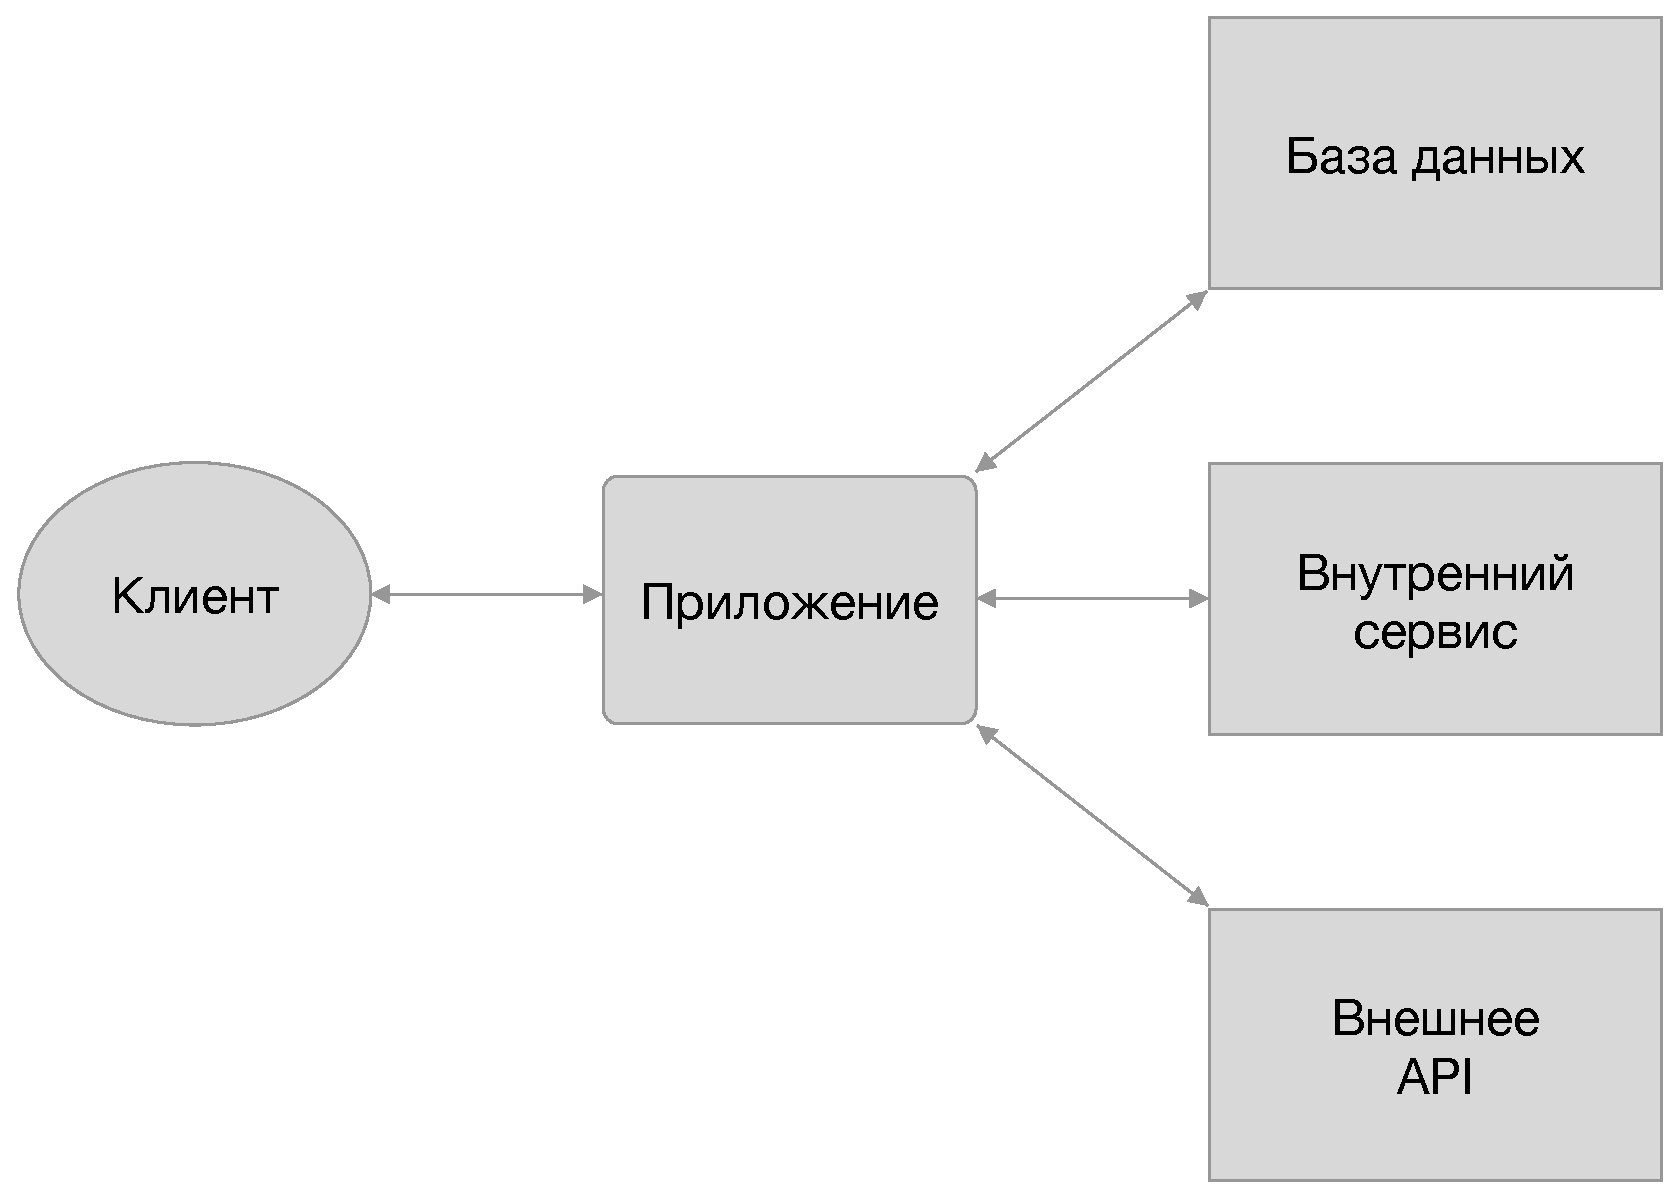
\includegraphics[width=\textwidth,height=\textheight,keepaspectratio]
    {img/service_diagram.eps}
\caption{Схема работы приложения в обычном режиме}
\label{fig:service_diagram}
\end{figure}

\subsection{Недостатки подхода}
Как упоминалось выше, при использовании TCP для мультиплексирования запросов,
или сохранении соединения с базой данных между запросами, подход к системе как
к ''черному ящику'' не работает в силу недетерминированности протокола обмена
сообщениями. Также безопасные соединения, устанавливаемые с помощью SSL/TLS
требуется расшифровывать в силу того, что данные основаны на случайных числах,
источник которых сложно повторить. По этим причинам механизм тестирования
подходит для ограниченного набора приложений, которые работают по достаточно
простым протоколам. В то время, как большинство современного ПО не
удовлетворяет данным критериям, заметное количество старых приложений можно
тестировать таким образом. Также тесты, генереруемые из больших файлов
захвата имеют больший риск ложноотрицательного результата в силу высокой
вероятности недетерминированного поведения системы.


\subsection{Выбор языка программирования}
Реализуемое в рамках данной работы приложение должно создавать много сетевых
соединений и обрабатывать множество сетевых соединений от тестируемого
сервиса. В качестве возможных языков, удобных для реализации приложения были
рассмотрены следующие решения:
\begin{itemize}
    \item C. В данном языке работа с множественными потоками на операционной
        системе Linux используется библиотека \lstinline{pthreads}, создающая
        реальные потоки на каждый внутренний поток приложения, что создает
        большие расходы на их переключение средствами ядра Linux. Также язык
        требует ручного управления памятью и созданием и удалением объектов
        синхронизации, увеличивая требуемое время на разработку и повышая
        сложность поддержки.  
    \item C++. В отличие от C, язык C++ более приспособлен к многопоточной
        работе, представляя готовые примитивы синхронизации, но все еще имеет
        ряд проблем с коммуникацией между каналами, используя для этого
        разделяемую память, что увеличивает риск состояний гонки и усложняет
        нахождение дефектов.  
    \item Go. Язык Go обладает сборкой мусора, позволяющей перенести
        ответственность за управление памятью на среду исполнения. Также язык
        позволяет исполнять несколько потоков приложения в рамках одного
        реального потока, что повышает производительность. В языке реализованы
        примитивы для взаимодействия между потоками в модели передачи сообщений,
        заметно упрощая разработку.  
\end{itemize}
По результатам проведенного сравнения был выбран язык программирования Go.
Дополнительным его преимуществом является полное статическое связывание с
кодом библиотек, упрощающее перенос приложения между системами и перенос его в
среду Docker.
\pagebreak

\section{Детали реализации}
\subsection{Формат хранения данных захвата}
По причине того, что тестируются приложения на старых версиях операционной
системы, на которых решения для сбора файла захвата, написанные на современных
языках программирования могут не запуститься по причине несовместимости
компилятора, необходимо использовать наиболее стандартное решения для перехвата
пакетов, реализация которого может быть доступна для наибольшего количества
версий операционной системы Linux. Единственным решением такого рода является
формат PCAP и библиотека libpcap для сбора пакетов с сетевых интерфейсов. Данный
формат хранит данные с минимальными накладными расходами, и размер такого файла
на несколько процентов больше, чем передаваемые по сети данные.  Для разбора
данных применяется библиотека \lstinline{gopacket}, являющаяся интерфейсом к
libpcap для языка программирования Go. Библиотека позволяет удобно обрабатывать
передаваемые по сети пакеты, абстрагируясь от их источника, что дает возможность
работать с трафиком как прямо в процессе сетевого взаимодействия (перехват на
лету), так и постфактум (из PCAP файла).  Для просмотра PCAP файлов в удобном
виде используется утилита Wireshark, отображающая содержимое пакетов в терминах
уровней модели OSI, давая информацию как про нижние уровни (MAC-адреса
устройств, IP-адреса и TCP/UDP порты), так и про данные на уровне приложения
(разбор протоколов MySQL, SMTP, DNS и так далее).

\subsection{Восстановление TCP-сессий}
TCP --- протокол обмена данными, устойчивый к потерям пакетов и их повреждению
при передаче по сети. В отличие от протокола UDP, который может не доставить
сообщение, доставить его повторно, или с большим опозданием, TCP обеспечивает
надежную передачу данных. С этим сопряжены заметные накладные расходы, например,
вызывающий множество споров процесс установки соединения (трехступенчатое
рукопожатие). Все это приводит к увеличению времени, требуемого на передачу
данных.

Еще одним важным отличием от протокола UDP является то, что в то время как UDP
передает датаграммы (сообщения с указанным размером), TCP передает поток данных.
Это существенно в целях восстановления переданных данных, так как запрос,
который на стороне приложения выглядит, как одно сообщение, по сети передается
как произвольный набор пакетов, часть из которых сетью отвергается по причине
ошибок или запоздания.

GoClown рассматривает любое взаимодействие приложения и внешнего сервиса как
последовательность запрос-ответ-запрос, что подразумевает превращение
захваченного трафика в линейный диалог. В этих целях используется библиотека
gopacket.tcpassembly, позволяющая выполнять многопоточную обработку и
восстановление потоков данных протокола TCP. На каждую сессию, определяемую
IP-адресом и портом сервера и клиета создается объект-обработчик. На любой
диалог создается два обработчика, по одному на направление обмена данными.
Пакеты потребляются сборщиком, который восстанавливает наборы байт TCP потоков,
и распределяет их по обработчикам, уведомляя их о начале и завершении потока.
Данная архитектура легко масштабируется и позволяет быстро восстанавливать
большие сессии.

\subsection{Фильтрация пакетов на уровне ядра Linux}
netfilter --- компонент ядра Linux, отвечающий за обработку и изменение сетевых
пакетов. Работает на втором и третьем уровне модели OSI, меняя пакеты на
основании исходящих и входящих IP-адресов, TCP/UDP портов и аппаратных адресов.
В качестве интерфейса к компоненту на уровне пользовательского пространства
ОС Linux используется утилита iptables, позволяющая просматривать и создавать
правила маршрутизации пакетов в системе.

iptables по умолчанию содержит следующие таблицы маршрутизации:
\begin{itemize}
\item filter --- таблица фильтрации. Она позволяет принимать или отклонять
пакеты на основе входящих/исходящих IP-адресов, MAC-адресов, TCP/UDP портов, а
также пересылать их на другой сетевой интерфейс.  
\item nat --- таблица преобразования сетевых адресов (Network address
translation). Она позволяет перенаправлять входящие и исходящие пакеты на
IP-адреса, отличные от изначальных, а также изменять TCP/UDP порты.  
\item mangle --- таблица преобразования служебных полей пакетов. Она позволяет,
например, изменять TTL пакетов.  
\item security --- таблица изменения маркировки безопасности пакетов и
соединений.  
\item raw --- таблица обработки сырых пакетов до их попадания в общую систему.  
\end{itemize}

Наиболее важной для обеспечения работы GoClown является таблица nat. В силу
того, что приложение может устанавливать соединение с некоторым IP-адресом,
прописанным прямо в его исходном коде, а не в виде доменного имени, возникает
необходимость перенаправлять такие соединения на GoClown. Для этого в таблице
NAT устанавливается правило переадресации пакетов с комбинации порта и IP-адреса,
найденного в журнале захвата пакетов, на порт и IP-адрес из сети 127.0.0.0/8.
Данная сеть выбрана по той причине, что, согласно стандарту RFC все адреса
из данной сети обслуживаются петлевым интерфейсом loopback, направляющим эти
соединения обратно на машину-хост, на которой запущено приложение \cite{rfc1122}
и GoClown, которое на данном адресе будет слушать входящие соединения.
Таким образом, если приложение попытается установить соединение с внешним
ресурсом, оно будет перенаправлено на GoClown, имитирующий его.

\subsection{Подделка доменных имен}
Помимо IP-адресов внешних сервисов, настроенных в приложении, приложение также
может использовать сервисы, разрешая их адреса по доменному имени. PCAP файл
содержит UDP-запросы к DNS-серверам, что позволяет найти список используемых
имен и IP-адресов, которые соответствовали им на момент записи пакетов,
и построить ассоциацию. На этапе тестирования GoClown создает свой DNS-сервер,
которые разрешает доменные имена на внутренние IP-адреса приложения.

\subsection{Комбинации IP-адрес:порт}
GoClown остлеживает все отправленные пакеты, в случае TCP взаимодействия
восстанавливая из сырых пакетных данных сессии. Любая такая сессия
рассматривается одним из четырех способов:
\begin{enumerate}
\item Соединение открывается с IP-адреса приложения, и направлено на IP-адрес
приложения. Это считается внутренним взаимодействием и игнорируется.  
\item Соединения открывается с IP-адреса приложения, и направлено на внешний
IP-адрес. Это считается исходящим соединением, и взаимодействие запоминается.
GoClown в данном случае будет выступать сервером.  
\item Соединение открывается с внешнего IP-адреса и направлено на IP-адрес
приложения. Это считается входящим соединением, и взаимодействие запоминается.
GoClown в данном случае будет выступать клиентом, открывающим соединение.  
\item Соединение открывается с внешнего IP-адреса и направлено на внешний
IP-адрес. Это считается внешним взаимодействием, захваченным случайно и
игнорируется.
\end{enumerate}

В случае, когда соединение запоминается, строится ацикличный конечный автомат.
Этот автомат определяет модель повтора взаимодействия.

При запуске GoClown в режиме активного тестирования производятся следующие
действия:
\begin{enumerate}
\item Создается DNS-cервер, который обслуживает приложение. Всем доменным
именам, которые запрашивались приложением ставится в соответствие уникальный
IP-адрес из сети 127.0.0.0/8.  
\item На каждый внешний сервис, с которым взаимодействовало приложение создается
сервер, слушающий подключения на IP-адресе из сети 127.0.0.0/8.  
\item С помощью утилиты iptables, предоставляющей доступ к компоненту ядра
netfilter устанавливается набор правил, переадресующий исходящие пакеты на
IP-адреса внешних сервисов на внутренние IP-адреса, обслуживаемые GoClown.  
\end{enumerate}

\subsection{Повтор данных}

\begin{figure}[H]
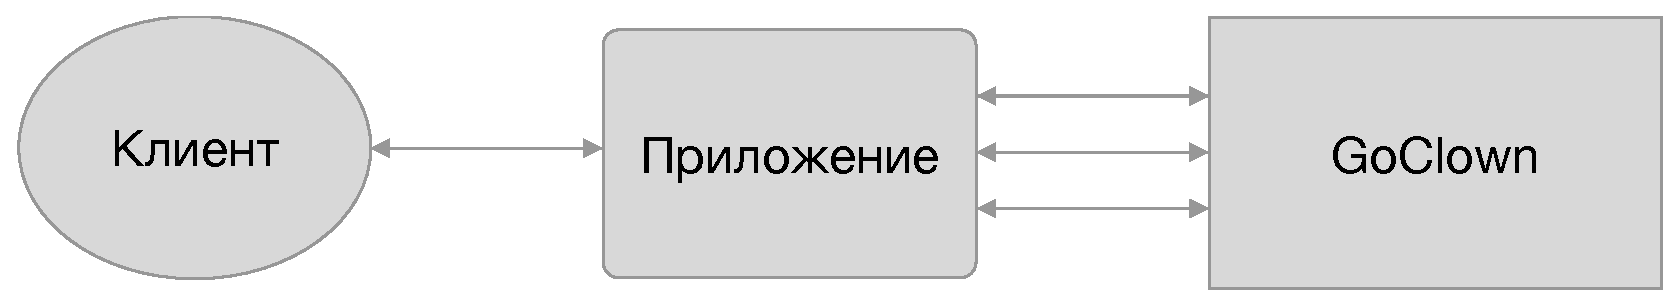
\includegraphics[width=\textwidth,height=\textheight,keepaspectratio]
    {img/service_diagram_clowned.eps}
\caption{Схема работы приложения во время работы GoClown}
\label{fig:service_diagram_clowned}
\end{figure}

При завершении подготовительного этапа тестируемое приложение можно запускать.
Далее приложение получает внешние запросы, идентичные тем, которые делались
на этапе захвата пакетов. Когда для их обработки приложение устанавливает
соединение и обменивается данными с внешними сервисами, их подменяет GoClown,
отвечая на запросы (при условии их полной идентичности таковым при захвате)
данными, которыми отвечал соответствующий внешний сервис. В случае, если
какой-то этап данного обмена проходит не так, как ожидается (например,
неожиданное закрытие соединения или ответ приложения, отличный от наблюдаемых
ранее), тестирование признается неудачным и процесс завершается.
Внутри приложение взаимодействие рассматривается как конечный автомат.
Пример такого автомата представлен на \autoref{fig:automata}.

\begin{figure}[h]
\begin{center}
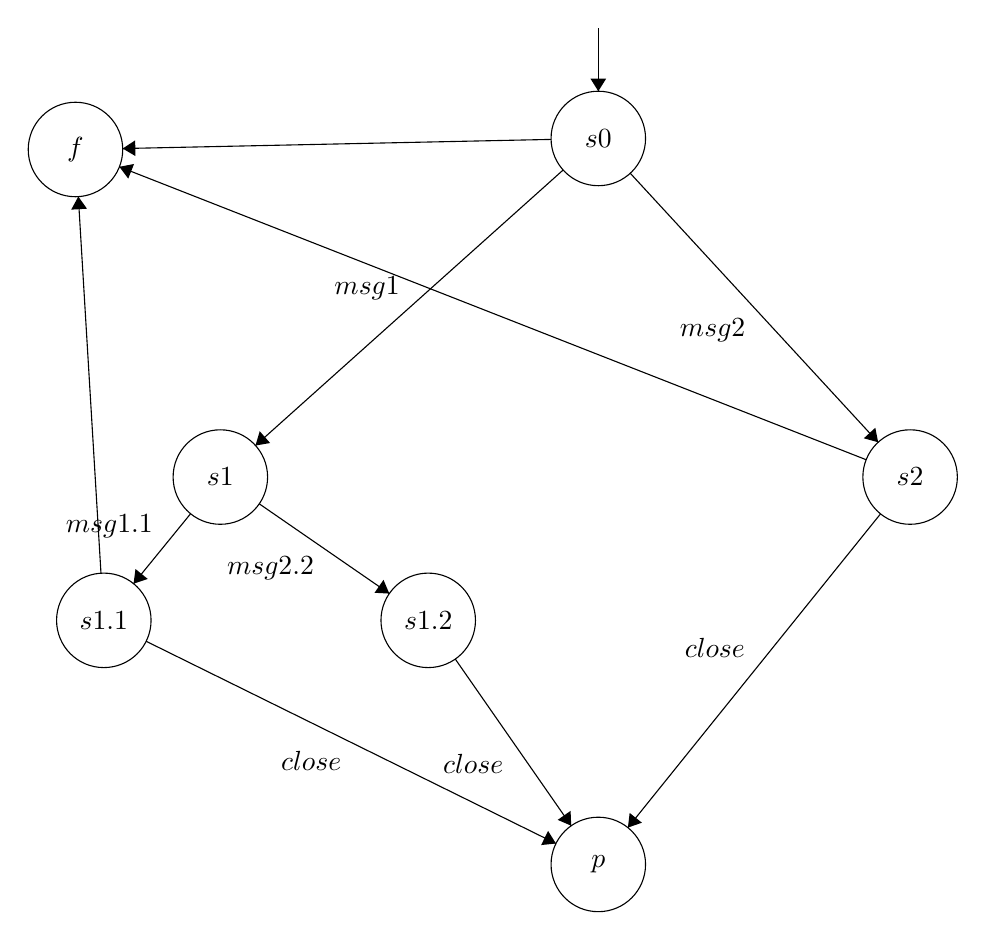
\begin{tikzpicture}[scale=0.2]
\tikzstyle{every node}+=[inner sep=0pt]
\draw [black] (16.2,-29.7) circle (3);
\draw (16.2,-29.7) node {$s1$};
\draw [black] (60,-29.7) circle (3);
\draw (60,-29.7) node {$s2$};
\draw [black] (40.2,-8.2) circle (3);
\draw (40.2,-8.2) node {$s0$};
\draw [black] (7,-8.9) circle (3);
\draw (7,-8.9) node {$f$};
\draw [black] (8.8,-38.8) circle (3);
\draw (8.8,-38.8) node {$s1.1$};
\draw [black] (29.4,-38.8) circle (3);
\draw (29.4,-38.8) node {$s1.2$};
\draw [black] (40.2,-54.3) circle (3);
\draw (40.2,-54.3) node {$p$};
\draw [black] (37.97,-10.2) -- (18.43,-27.7);
\fill [black] (18.43,-27.7) -- (19.36,-27.54) -- (18.7,-26.79);
\draw (25.52,-18.46) node [above] {$msg1$};
\draw [black] (42.23,-10.41) -- (57.97,-27.49);
\fill [black] (57.97,-27.49) -- (57.79,-26.57) -- (57.06,-27.24);
\draw (49.57,-20.41) node [left] {$msg2$};
\draw [black] (37.2,-8.26) -- (10,-8.84);
\fill [black] (10,-8.84) -- (10.81,-9.32) -- (10.79,-8.32);
\draw [black] (57.21,-28.6) -- (9.79,-10);
\fill [black] (9.79,-10) -- (10.35,-10.75) -- (10.72,-9.82);
\draw [black] (40.2,-1.2) -- (40.2,-5.2);
\fill [black] (40.2,-5.2) -- (40.7,-4.4) -- (39.7,-4.4);
\draw [black] (14.31,-32.03) -- (10.69,-36.47);
\fill [black] (10.69,-36.47) -- (11.59,-36.17) -- (10.81,-35.54);
\draw (11.94,-32.82) node [left] {$msg1.1$};
\draw [black] (18.67,-31.4) -- (26.93,-37.1);
\fill [black] (26.93,-37.1) -- (26.56,-36.23) -- (25.99,-37.05);
\draw (19.38,-34.75) node [below] {$msg2.2$};
\draw [black] (8.62,-35.81) -- (7.18,-11.89);
\fill [black] (7.18,-11.89) -- (6.73,-12.72) -- (7.73,-12.66);
\draw [black] (58.12,-32.04) -- (42.08,-51.96);
\fill [black] (42.08,-51.96) -- (42.97,-51.65) -- (42.19,-51.03);
\draw (49.54,-40.57) node [left] {$close$};
\draw [black] (31.12,-41.26) -- (38.48,-51.84);
\fill [black] (38.48,-51.84) -- (38.44,-50.9) -- (37.62,-51.47);
\draw (34.2,-47.91) node [left] {$close$};
\draw [black] (11.49,-40.13) -- (37.51,-52.97);
\fill [black] (37.51,-52.97) -- (37.01,-52.17) -- (36.57,-53.07);
\draw (21.97,-47.06) node [below] {$close$};
\end{tikzpicture}
\caption{Устройство конечного автомата диалога}
\label{fig:automata}
\end{center}
\end{figure}

Здесь s0 --- начальное состояние сервера-имитатора. Функцией перехода является
хеш-функция данных, полученных от тестируемого приложения. Если в текущем
состоянии нет соответствующего хеша, то происходит переход в состояние f,
обозначающее тест, завершенный с ошибкой. Например, если передать msg2, а после
него msg1.1, тест не будет считаться пройденным. Если же обмен данными
завершается успешно и соединение закрывается (переход close) в состоянии, в
котором это является допустимым переходом, происходит переход в состояние p,
обозначающее успешное прохождение теста.
Использование хешей в качестве функции перехода позволяет двукратно уменьшить
потребление оперативной памяти. Также представление взаимодействия в виде
дерева дает возможность уменьшить потребление памяти еще больше при
использовании Б-Дерева, которое удобно хранить на жестком диске, загружая
в оперативную память только нужные его части.

\subsection{Пользовательский интерфейс}
Для удобства интеграции инструмента в процессы автоматической сборки и
тестирования приложение использует текстовый интерфейс.
Приложение реализует следуюшие подкомманды:

\begin{itemize}
    \item \lstinline{goclown replay} --- запуск тестового сервера,  
    \item \lstinline{goclown list\_sessions} --- вывод списка сессий,  
    \item \lstinline{goclown extract\_tree} --- вывод конечных автоматов,  
    \item \lstinline{goclown reroute} --- перенаправление TCP-адреса на
        локальный адрес.  
\end{itemize}

\subsubsection{Вывод списка сессий}
Команда \lstinline{goclown list_sessions} выводит все двунаправленные
TCP-взаимодействия, обнаруженные в переданном файле PCAP. Команда используется
для определения, какие IP-адреса используются приложением для установления
соединений. Пример использования команды представлен на
\autoref{fig:listsessions}. В данном случае команде был передан файл
взаимодействия с тестовым сервисом внутри Docker, имеющим IP-адрес
\lstinline{172.19.0.2}, принимающим HTTP-запросы, отправленные на порт 8080, и
взаимодействующий с базой данных, имеющей IP-адрес \lstinline{172.19.0.3},
принимающей TCP-соединения на 3306 порту. По данному выводу можно определить,
что соединение с базой данных устанавливается всего один раз, и что было
отправлено 4 HTTP-запроса. Так как каждый HTTP-запрос требует для обработки
обращение к базе данных, можно сделать вывод, что соединение с ней
переиспользуется.

\begin{figure}[H]
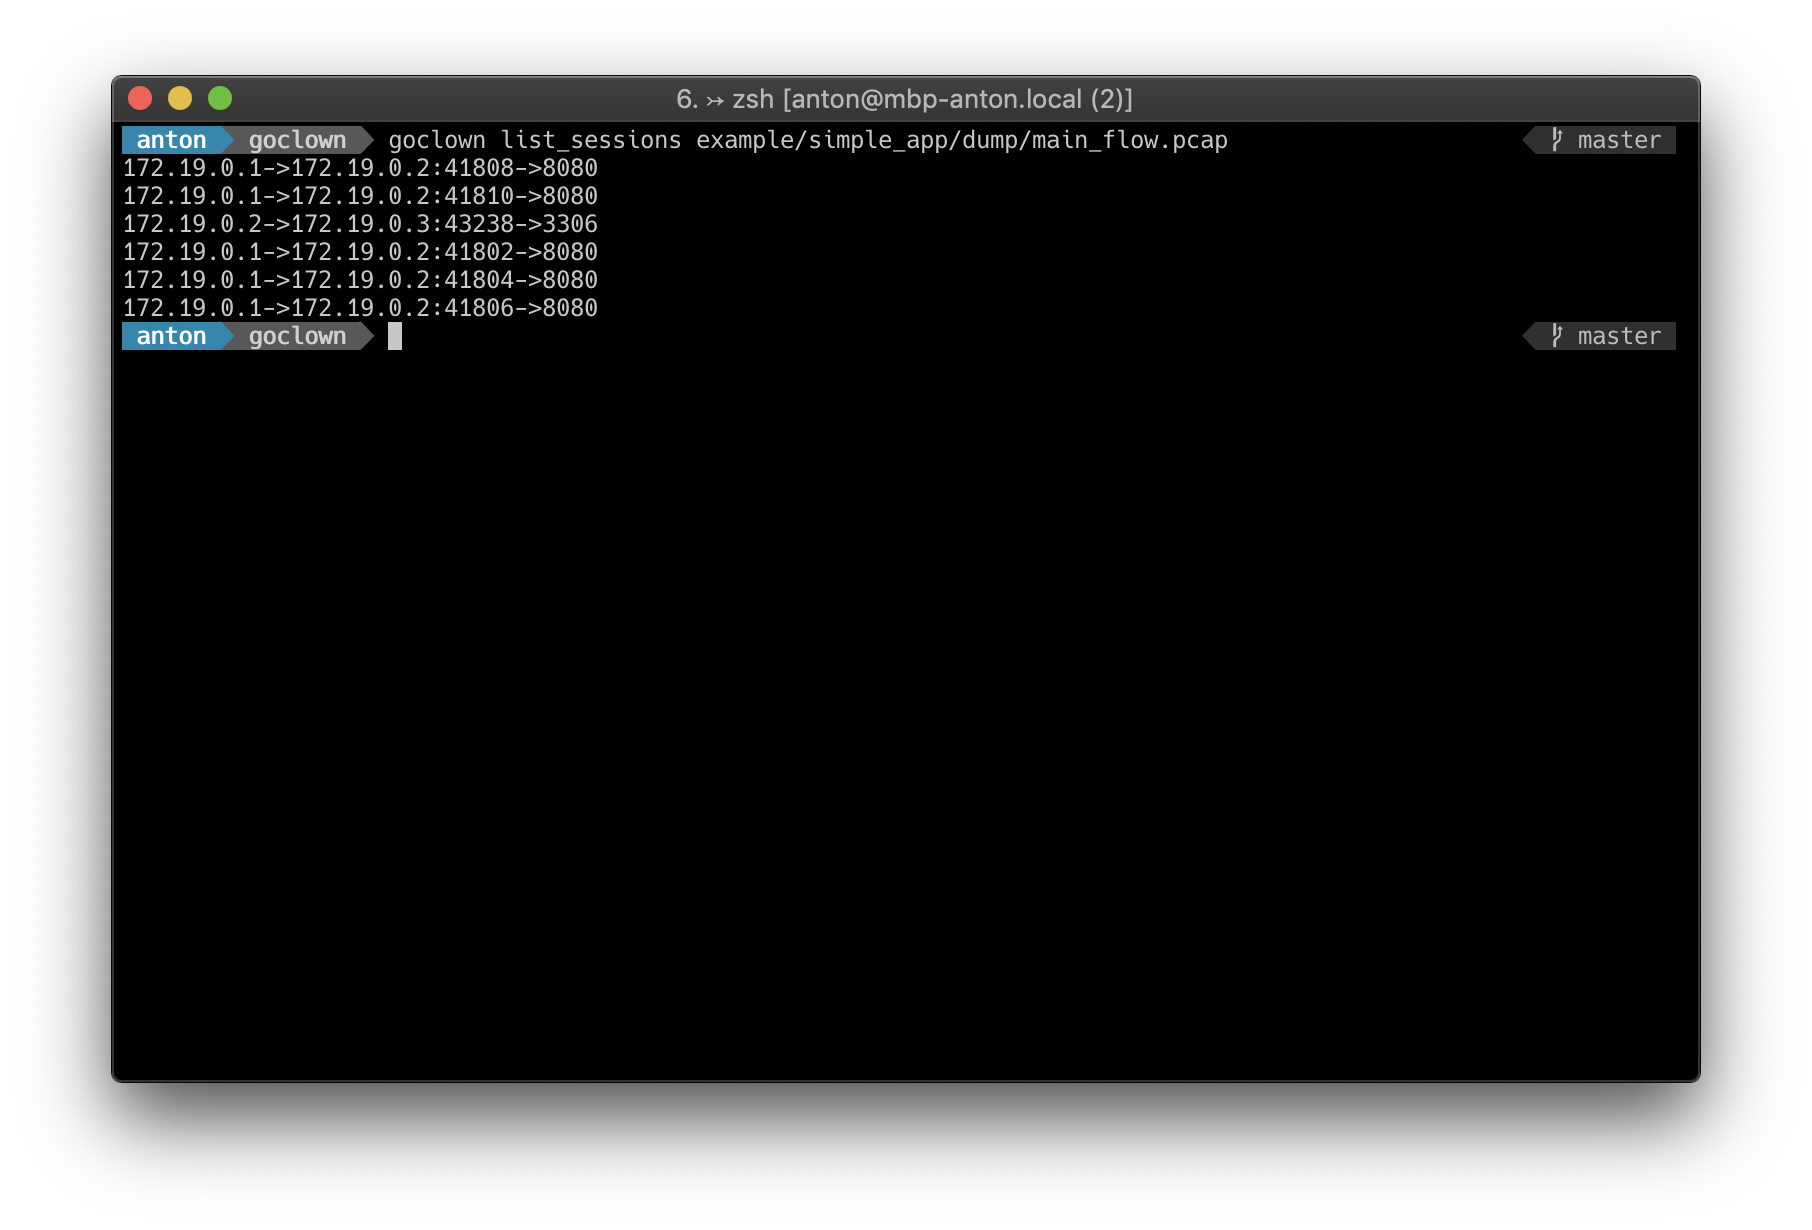
\includegraphics[width=\textwidth,height=\textheight,keepaspectratio]
    {img/list_sessions.png}
\caption{Пример команды list\_sessions}
\label{fig:listsessions}
\end{figure}

\subsubsection{Вывод конечных автоматов}
Команда \lstinline{goclown extract_tree} принимает на вход PCAP файл, и адреса,
которые имеет приложение, и создает все конечные автоматы, в которых инициатором
соединения являлся один из этих IP-адресов, а принимающей стороной --- внешний
сервис, то есть сервис с IP-адресом, отличным от переданных. Чтобы получить
такой список адресов рекомендуется использовать команду
\lstinline{goclown list_sessions}. Конечный автомат выводится в формате JSON,
где ключами корневого словаря являются комбинации IP-адрес и порт адресата
соединения, а значениями -- конечные автоматы. Пример представлен на
\autoref{fig:extracttree}. По данному выводу можно определить, что одним из
адресатов являлся сервис базы данных, из того, что в изначальном состоянии
автомата \lstinline{data} не определен можно сказать, что сервер не отвечает
приветствием. Далее можно видеть, соответствие md5 хэша запроса и ответа. В
данном случае извлекался только один диалог в силу переиспользования соединения
с базой данных, поэтому дерево имеет вид бамбука.

\begin{figure}[H]
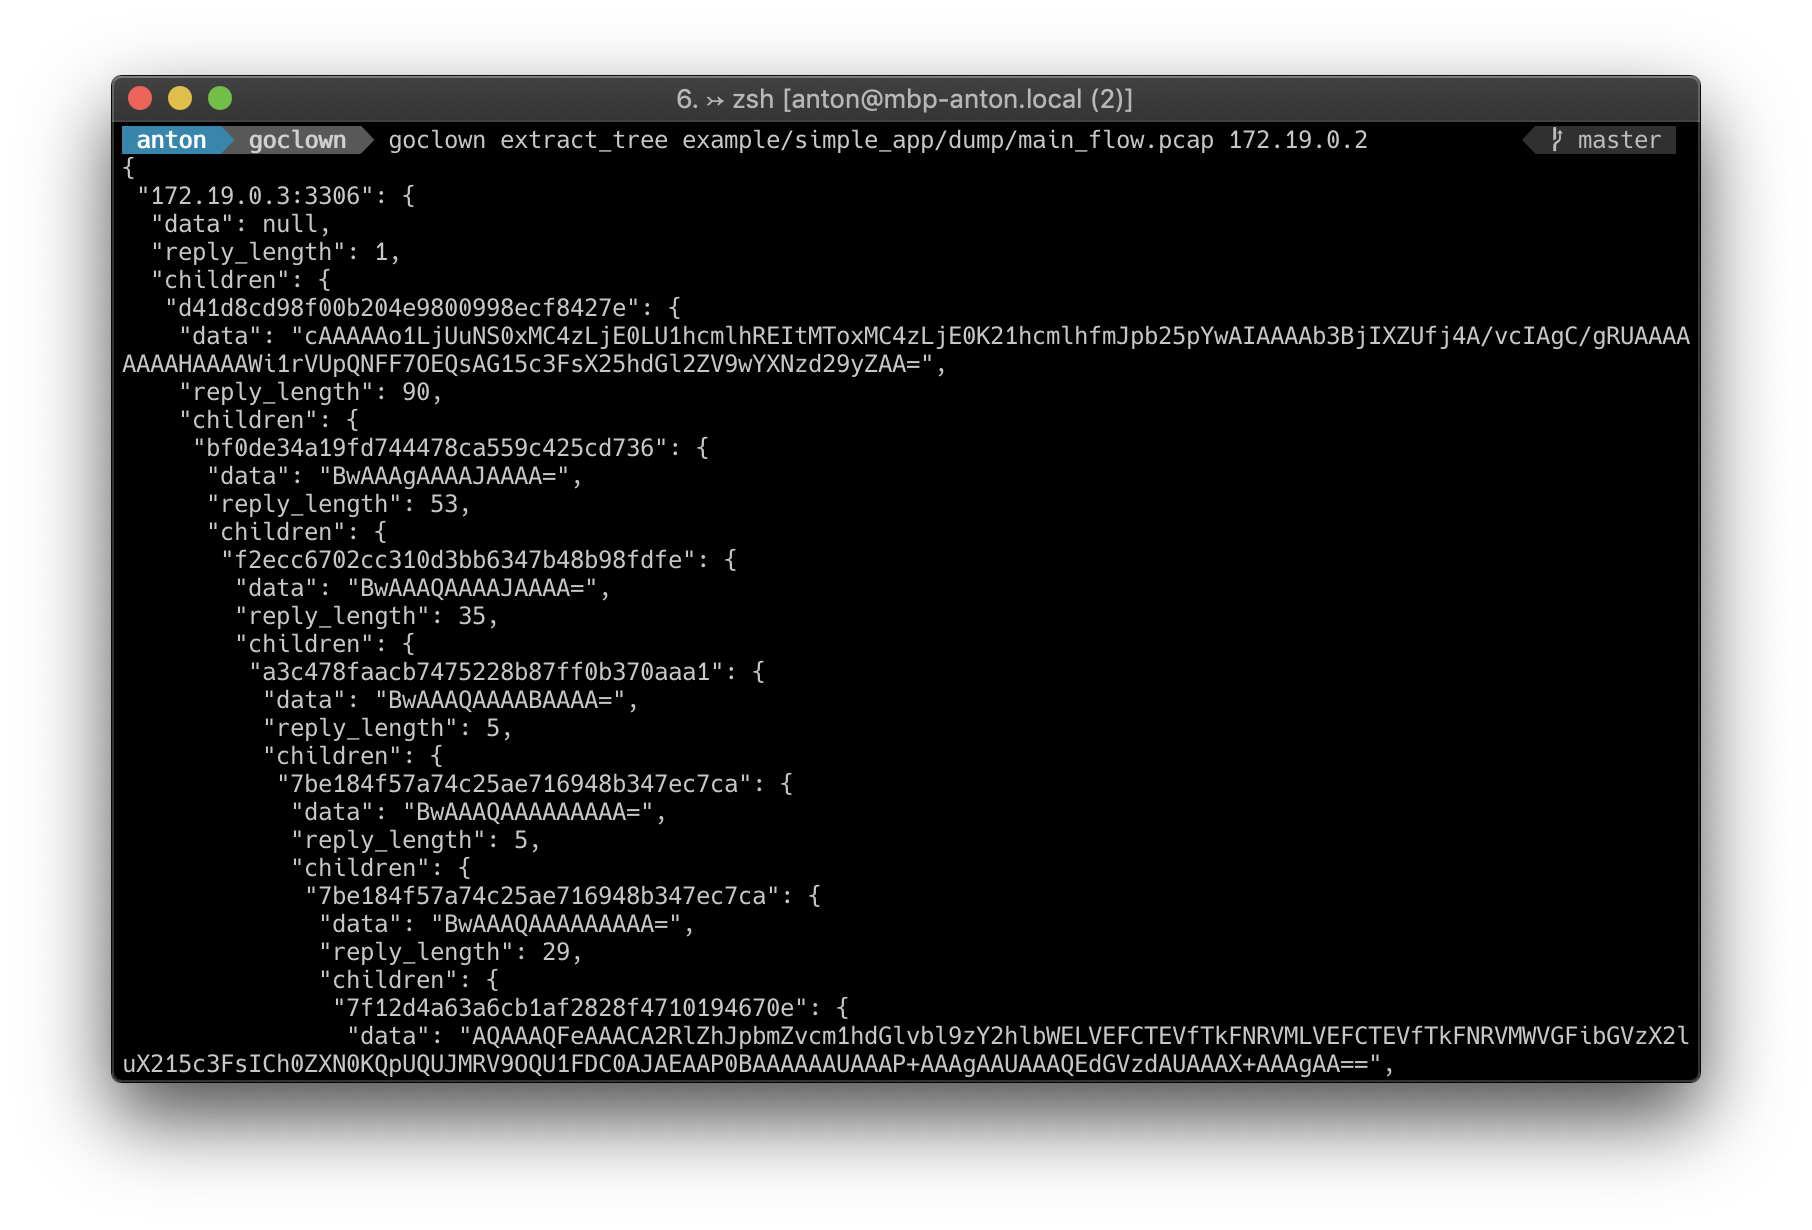
\includegraphics[width=\textwidth,height=\textheight,keepaspectratio]
    {img/extract_tree.png}
\caption{Пример команды extract\_tree}
\label{fig:extracttree}
\end{figure}

\subsubsection{Перенаправление TCP-запросов}
Команда \lstinline{goclown reroute} принимает на вход IP-адрес и порт, и
совершает модификацию таблиц фильтрации трафика iptables для того, чтобы
исходящие соединения на этот адрес перенаправлялись обратно на локальный адрес.
Команда возвращает адрес, на которой производится переадресация. Пример
представлен на \autoref{fig:reroute}. В данном случае происзодит переадресация
с \lstinline{192.168.0.1:3000} на \lstinline{127.0.0.2:1000}. Это значит, что
если создать сервер, слушающий входящие соединения на адресе
\lstinline{127.0.0.2:1000}, то любое исходящее соединение на адрес
\lstinline{192.168.0.1:3000} будет им принято и обработано.

\begin{figure}[H]
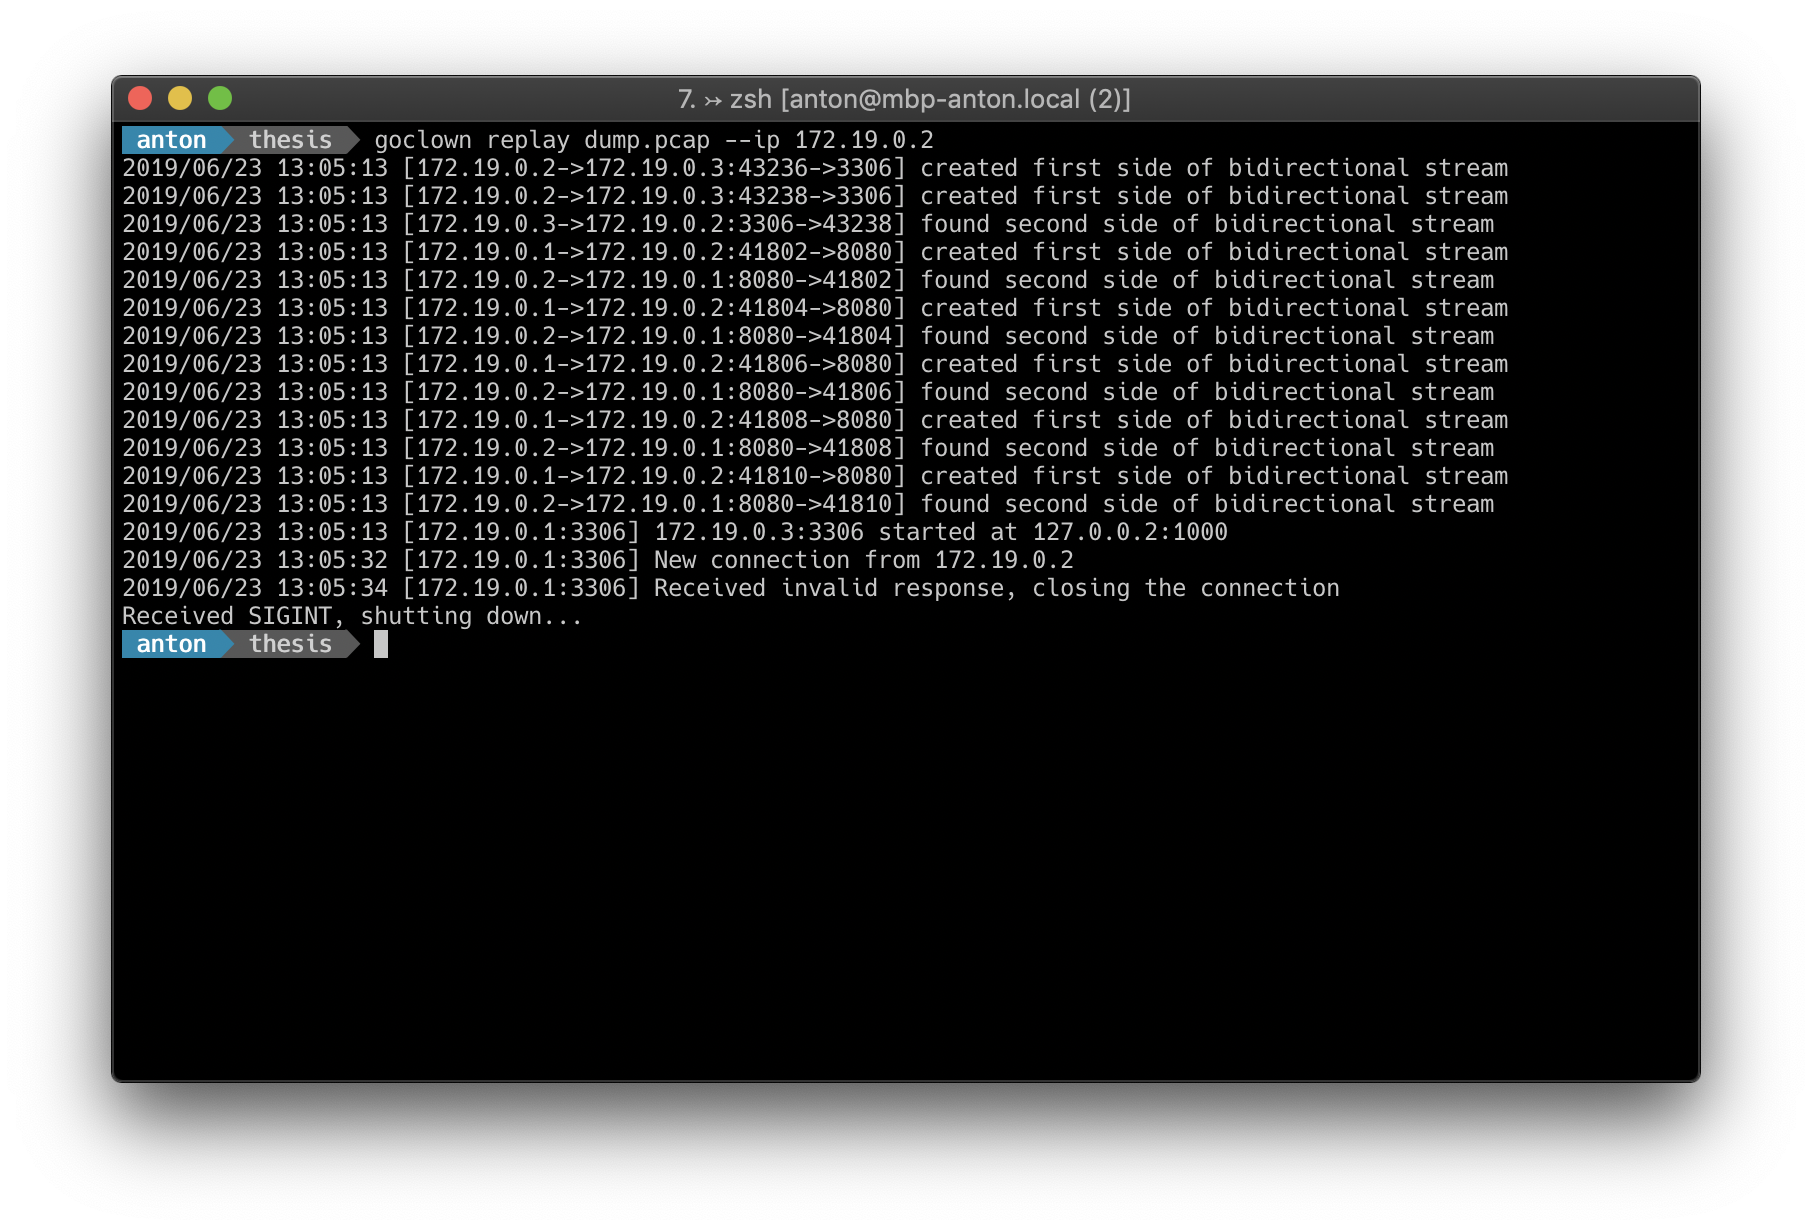
\includegraphics[width=\textwidth,height=\textheight,keepaspectratio]
    {img/reroute.png}
\caption{Пример команды reroute}
\label{fig:reroute}
\end{figure}

\subsubsection{Запуск тестового сервера}
Команда \lstinline{goclown replay} принимает на вход PCAP файл и адреса, которые
имеет приложения. Она извлекает конечные автоматы и создает на каждого
найденного адресата отдельный сервер, отвечающий в соответствии с его автоматом.
В случае обнаружения несоовтветствия, в систему сообщений выводится ошибка и
соединение закрывается. Пример запуска команды можно видеть на
\autoref{fig:replay}. В исходный код приложения были внесены изменения, чтобы
его взаимодействие отличалось от записанного ранее. Таким образом, оно отправило
запрос, не являющийся известным для сервера, из-за чего он разорвал подключение.

\begin{figure}[H]
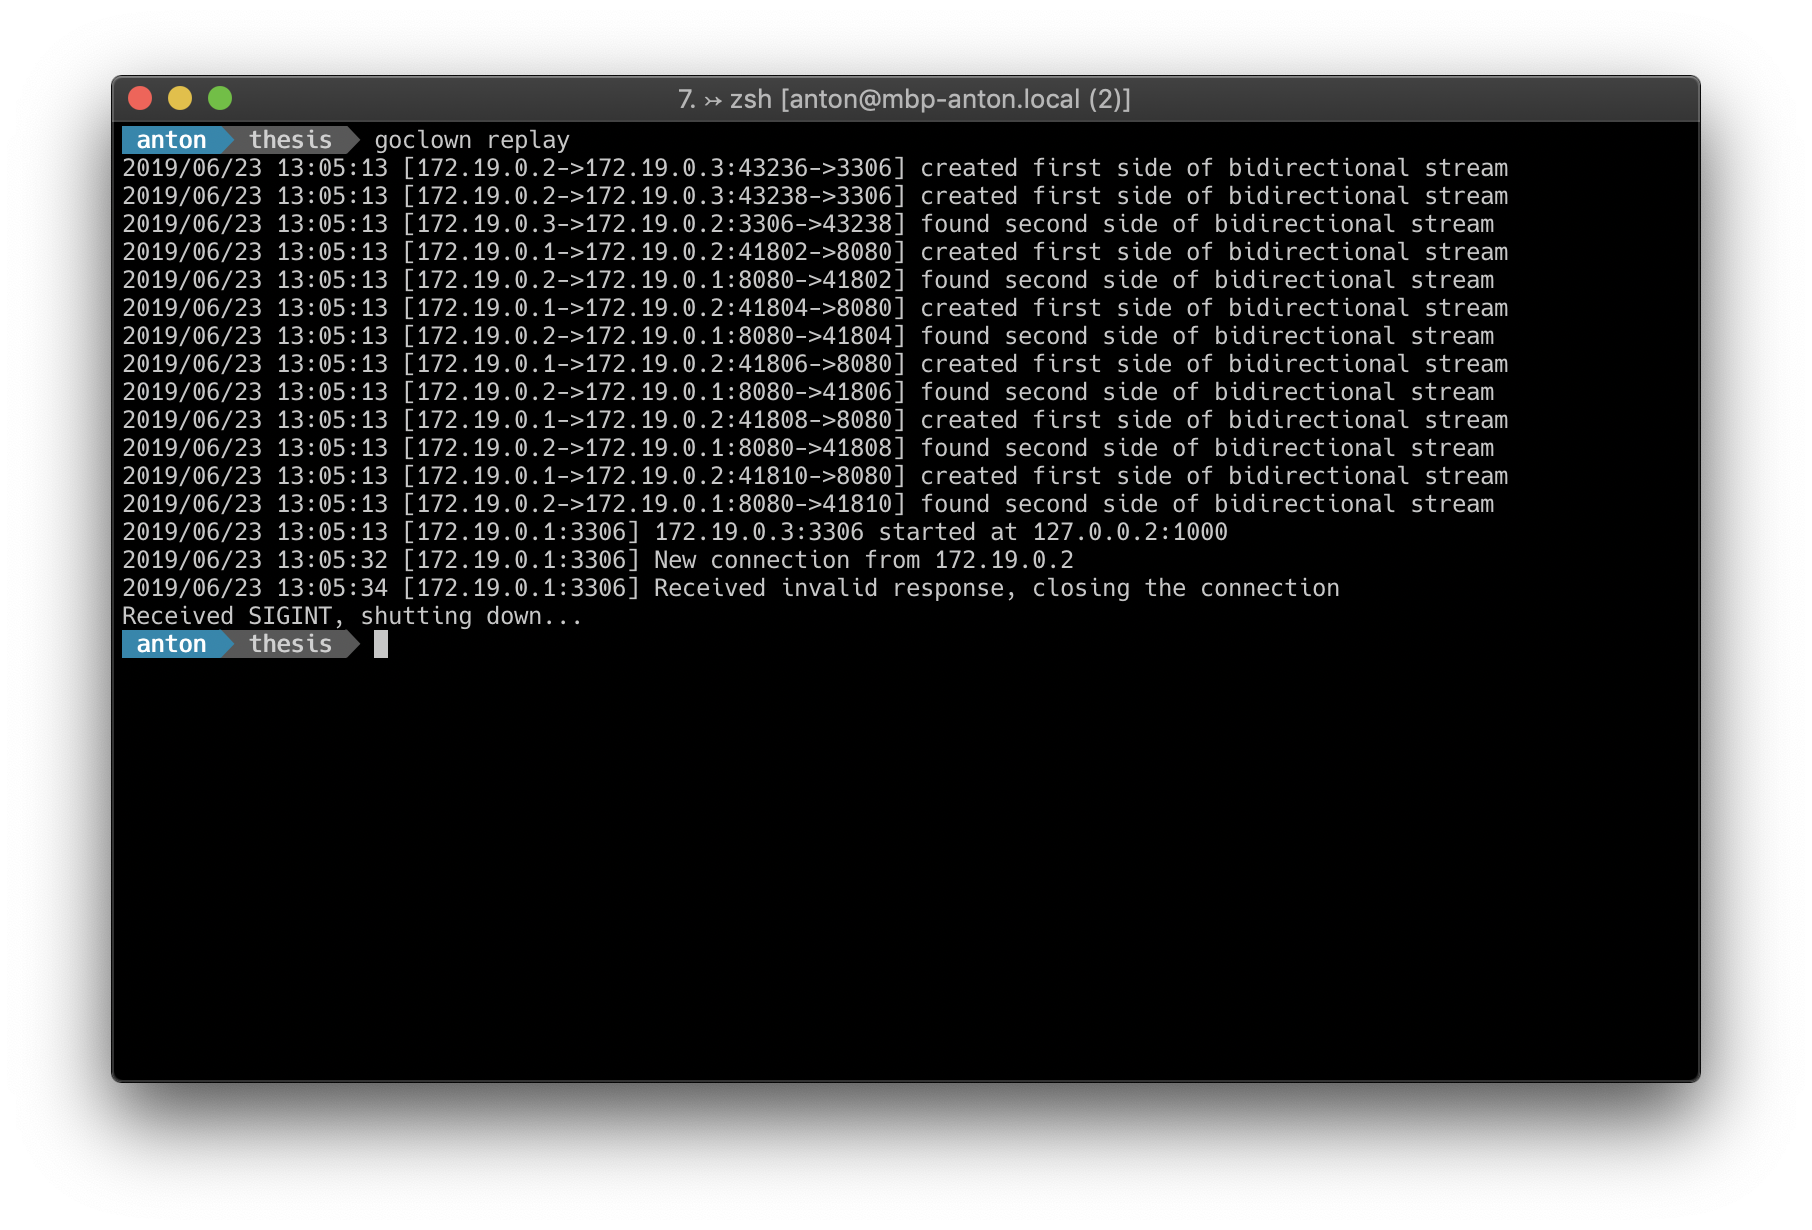
\includegraphics[width=\textwidth,height=\textheight,keepaspectratio]
    {img/replay.png}
\caption{Пример команды replay}
\label{fig:replay}
\end{figure}


\pagebreak

\section{Проверка работоспособности}
\subsection{Автоматическое тестирование}
Все компоненты GoClown покрыты тестами, проверяющими, что поведение каждого
модуля в отдельности соответствует ожиданиям. Для компонентов, которые
в том или ином виде взаимодействуют с захваченными пакетами используются
данные, полученные с тестового стенда (см. ниже). Это позволяет приблизить
тестовое окружение к реальному, но разработка тестов происходит не по принципам
TDD, согласно которым тесты должны описывать ожидаемую семантику на очевидных
примеров, так как какое-то поведение приложения фиксируется как корректное
(после ручной проверки), и закрепляется в тестах, как ожидаемое. Также тесты
становятся менее прозрачными, потому что недостаточно прочитать их исходный код,
но дополнительно требуется изучить файл с захваченными пакетами с помощью
программы-анализатора, наподобии Wireshark. Стоит заметить, что данная проблема
характерна для большинства приложений, так или иначе разбирающих не
человекочитаемый формат файлов, что видно на примере тестов библиотеки
gopacket.

\subsection{Практическое тестирование}
В качестве объекта тестирования при разработке было написано простое приложение
на ЯП Python, которое реализовывало примитивный интерфейс к списку строчек,
хранимому в базе данных.
Доступные HTML методы:
\begin{enumerate}
\item \lstinline{POST /create_table/} --- создать таблицу для хранения строк  
\item \lstinline{POST /append_string/} --- добавить тело запроса как строку  
\item \lstinline{GET /strings/} --- получить список строк  
\item \lstinline{POST /delete_table/} --- удалить таблицу со строками  
\end{enumerate}
Каждый из запросов порождает отдельное соединение с базой данных для получения
данных или их изменения.
На это приложение был направлен небольшой набор запросов, и все сетевые
взаимодействия были записаны с помощью утилиты tcpdump, создающей PCAP файл,
требуемый для работы GoClown.

\subsection{Апробация}
Пример, приведенный выше, может показать качество работы приложения в случае,
когда отсутствуют заметные потери пакетов, и запросы достаточно просты.
Для проверки приложения в тех условиях, для которых оно было разработано,
используется повторение скриптов синхронизации.
Внутренний сервис компании Acronis, отвечающий за хранение и обработку данных
пользовательских учетных записей, включая их личную информацию и информацию
о приобретенных продуктах представляет собой очень большую систему, включающую
в себя несколько десятков различных компонентов, в том числе большое число
скриптов синхронизации и обработки данных, включающихся по расписанию. Они
нередко выполняются на специально отведенных в таких целях виртуальных машинах.
Чтобы записать сетевое взаимодействие одного такого скрипта, а не всех,
запущенных с ним на одном сервере, была клонирована виртуальная машина, его
содержащая, и отключен запуск задач по расписанию. С помощью инструмента
tcpdump были захвачены все сетевые взаимодействия скрипта в PCAP файл.
Далее в среде Docker этот же скрипт был запущен, но с заменой сетевого
взаимодействия на его имитацию с помощью GoClown. Работоспособность приложения
не нарушилась, и все запросы к базе данных и серверу отправки электронной почты
были совершены успешно, что говорит о том, что GoClown выполняет поставленную
задачу.
